\documentclass[12pt]{article}

% === Packages ===
\usepackage[utf8]{inputenc}
\usepackage[T1]{fontenc}
\usepackage{lmodern}
\usepackage[margin=1in]{geometry}
\usepackage{amsmath,amssymb}
\usepackage{graphicx}
\usepackage{booktabs}
\usepackage{tabularx}
\usepackage{xcolor}
\usepackage[round]{natbib}
\usepackage[colorlinks=true,linkcolor=blue!60!black,citecolor=blue!60!black,urlcolor=blue!60!black]{hyperref}
\usepackage{microtype}
\usepackage{setspace}
\usepackage{parskip}

% === Formatting ===
\onehalfspacing

% === Title ===
\title{The Four-Model Theory of Consciousness:\\A Simulation-Based Framework Unifying the Hard Problem, Binding, and Altered States}
\author{Matthias Gruber\\
\textit{Independent researcher}\\
\texttt{matthias@matthiasgruber.com}}
\date{}

% === Document ===
\begin{document}
\maketitle

\begin{abstract}
The science of consciousness remains in a pre-paradigm state, with no theory simultaneously satisfying the eight core requirements a complete theory must meet: the Hard Problem, the Explanatory Gap, the Boundary Problem, the Structure of Experience, Unity and Binding, Combination and Emergence, the Causal Role, and the Meta-Problem. I present the Four-Model Theory, in which consciousness is constituted by real-time self-simulation across four nested models arranged along two axes---scope (world vs.\ self) and mode (implicit vs.\ explicit). The implicit models (Implicit World Model, Implicit Self Model) are substrate-level, learned, and non-conscious. The explicit models (Explicit World Model, Explicit Self Model) are virtual, transient, and phenomenal---they are the simulation in which experience occurs. The theory's central claim is that qualia are virtual: they are the way the simulated self perceives its own states within the simulation, not properties of the physical substrate. This dissolves the Hard Problem by showing that ``Why does physical processing feel like something?'' commits a category error---the physical processing does not feel; the simulation does, and within the simulation, qualia are constitutive. Combined with a criticality requirement (the substrate must operate at the edge of chaos), the theory derives diverse phenomena from five principles: criticality, virtual qualia, a redirectable Explicit Self Model, variable implicit--explicit permeability, and virtual model forking. These principles unify psychedelic phenomenology, anesthetic mechanisms, dream states, split-brain phenomena, dissociative identity disorder, and animal consciousness. A systematic comparison shows the theory addresses all eight requirements. Nine novel testable predictions are offered, including that psychedelic ego dissolution content is controllable via sensory input and that psychedelics should alleviate anosognosia---predictions no competing theory generates. The criticality requirement, independently derived from Wolfram's computational framework in 2015, converges with empirical criticality literature consolidated in 2025--2026 \citep{HengenShew2025,AlgomShriki2026}---a decade-apart convergence from theoretical and empirical starting points.
\end{abstract}

\noindent\textbf{Keywords}: consciousness, hard problem, self-model, simulation, qualia, criticality, binding problem, altered states, psychedelics, substrate independence

%=============================================================================
\section{Introduction}
%=============================================================================

\subsection{The Pre-Paradigm State of Consciousness Science}

After three decades of intensive scientific investigation, consciousness research finds itself at an impasse. The field possesses no dominant paradigm in the Kuhnian sense \citep{Kuhn1962}, no agreed-upon methodology for linking subjective experience to objective measurement, and no theory that commands broad assent. Multiple frameworks compete for explanatory primacy---Integrated Information Theory (IIT; \citealp{Tononi2004}; \citealp{Albantakis2023}), Global Neuronal Workspace (GNW; \citealp{Baars1988}; \citealp{Dehaene2011}), Higher-Order Theories (HOT; \citealp{Rosenthal2005}; \citealp{Lau2011}), Predictive Processing (PP; \citealp{Friston2010}; \citealp{Seth2021}), Attention Schema Theory (AST; \citealp{Graziano2013}), Recurrent Processing Theory (RPT; \citealp{Lamme2006,Lamme2010}), and others---yet none has established decisive empirical or theoretical superiority over its rivals.

Recent developments have deepened the crisis rather than resolving it. The COGITATE adversarial collaboration published equivocal results in \textit{Nature} \citep{Melloni2023,COGITATE2025}: neither IIT nor GNW was fully confirmed, and the data favored posterior cortical involvement over either camp's predictions. A letter signed by over 100 researchers declared IIT pseudoscientific \citep{NatNeuro2025IIT}, provoking fierce rebuttals \citep{Konstantinou2025}. Reviews published in 2024--2025 have asked whether the field is making genuine progress or merely accumulating incompatible frameworks.

This paper argues that the impasse persists because no existing theory simultaneously addresses all of the fundamental requirements that a complete theory of consciousness must meet. Each theory excels on some requirements but remains silent on, or weak against, others. The field needs a framework that addresses the full set of challenges---not just neural correlates or access conditions, but the deep philosophical problems that make consciousness uniquely difficult.

\subsection{What Would Count as Progress?}

I propose that any theory claiming to provide a comprehensive account of consciousness must address eight core requirements, drawn from the philosophical and scientific literature. These requirements are not novel; each has been identified by previous authors as a central challenge (sources are given in Section~2). What is novel is the demand that a single theory address all eight simultaneously:

\begin{enumerate}
\item \textbf{The Hard Problem} \citep{Chalmers1995}---Why does physical processing give rise to subjective experience?
\item \textbf{The Explanatory Gap} \citep{Levine1983}---Why does the explanation of neural correlates feel incomplete?
\item \textbf{The Boundary Problem} \citep{Bayne2010,Tononi2004}---Where does the conscious system end?
\item \textbf{The Structure of Experience} \citep{Nagel1974}---How does physical processing produce richly structured experience?
\item \textbf{Unity and Binding} \citep{Treisman1980,Revonsuo1999}---How are distributed processes unified into coherent experience?
\item \textbf{Combination and Emergence} \citep{Chalmers2016}---How do non-conscious elements combine to produce consciousness?
\item \textbf{The Causal Role} \citep{Jackson1982}---Does consciousness do anything?
\item \textbf{The Meta-Problem} \citep{Chalmers2018}---Why do we think there is a hard problem?
\end{enumerate}

Section~2 develops each requirement in detail and surveys how existing theories fare against them. The remainder of the paper presents a theory---the Four-Model Theory---that, I argue, addresses all eight.

\subsection{Overview and Historical Context}

The Four-Model Theory was originally published in German as \textit{Die Emergenz des Bewusstseins} \citep{Gruber2015} and has been refined through a structured adversarial challenge process in 2026. The theory self-identifies as an intersection of Dennett's Multiple Drafts Model \citep{Dennett1991}, Metzinger's Self-Model Theory of Subjectivity \citep{Metzinger2003,Metzinger2009}, and neural network architecture. It is substrate-independent: the six-layer mammalian cortex is understood as an evolutionary implementation, not a requirement.

The theory proposes that consciousness consists of a real-time self-simulation running on an implicit (substrate-level) knowledge base. Qualia---the subjective ``feel'' of experience---are virtual: they exist within and are constitutive of the simulation, but do not exist at the substrate level. This two-level ontology dissolves the Hard Problem by showing it rests on a category error.

Combined with a criticality requirement derived independently from Wolfram's computational framework \citep{Wolfram2002}, the theory generates nine novel testable predictions and unifies phenomena across psychopharmacology, clinical neurology, sleep science, and comparative cognition under five principles.

The paper proceeds as follows. Section~2 establishes the eight requirements. Section~3 presents the Four-Model Theory. Sections~4 and~5 develop the philosophical commitments and the binding/criticality framework. Section~6 demonstrates the theory's explanatory range. Section~7 provides a systematic comparative analysis against major competitors. Section~8 presents the nine predictions. Sections~9--11 address open questions, implications, and conclusions.

%=============================================================================
\section{Eight Requirements for a Theory of Consciousness}
%=============================================================================

This section develops each of the eight requirements and briefly notes how current theories address or fail to address them. A detailed theory-by-theory comparison follows in Section~7; the purpose here is to establish the evaluative framework.

\subsection{The Hard Problem}

\citet{Chalmers1995,Chalmers1996} formulated the Hard Problem as the question of why physical processing is accompanied by subjective experience. We can explain all the \textit{functions} of consciousness---discrimination, integration, reporting, attention---without explaining why there is ``something it is like'' \citep{Nagel1974} to undergo these processes. The explanatory challenge is not about identifying neural correlates but about understanding why correlates are accompanied by phenomenality at all.

Most neuroscientific theories of consciousness (GNW, RPT, PP) focus on functional or mechanistic accounts and remain explicitly or implicitly silent on the Hard Problem. IIT attempts to address it by defining consciousness as intrinsic causal power ($\Phi$), treating experience as identical to integrated information---but this requires accepting panpsychist commitments that many find problematic \citep{Aaronson2014,Doerig2019}. HOT and AST offer deflationary accounts that explain \textit{why we report} having phenomenal experience but leave open whether they have truly addressed the phenomenality itself. Illusionism \citep{Dennett1991,Frankish2016} dissolves the problem by denying that qualia as traditionally conceived exist---a position that remains deeply controversial.

\subsection{The Explanatory Gap}

\citet{Levine1983} identified the Explanatory Gap as a distinct problem from the Hard Problem: even if we identify every neural correlate of every conscious state, the explanation seems to leave something out. The gap is between the third-person description (neural firing patterns) and the first-person reality (what the experience is like). \citet{Block1995,Block2007} further refined this as the distinction between access consciousness (the functional role) and phenomenal consciousness (the subjective feel).

The Explanatory Gap is often treated as a restatement of the Hard Problem, but it has a distinct character: it is about the \textit{form} of explanation rather than the \textit{existence} of the phenomenon. A theory that dissolves the Hard Problem should simultaneously close the Explanatory Gap.

\subsection{The Boundary Problem}

Where does the conscious system begin and end? Within the brain, only some processing is conscious at any given moment. Between organisms, it is unclear where to draw the line. The Boundary Problem asks for a principled account of what delineates conscious from non-conscious processing \citep{Bayne2010,Tononi2004}.

IIT provides the strongest existing treatment of this requirement through its exclusion postulate: the system with maximum $\Phi$ defines the boundary of consciousness. However, the computational intractability of calculating $\Phi$ limits its practical application. GNW defines conscious access in terms of global broadcasting, but the boundary between broadcast and non-broadcast content is not always sharp. PP uses Markov blankets \citep{Friston2010} but has been criticized for being too liberal in its boundary-setting \citep{Bruineberg2022}.

\subsection{The Structure of Experience}

Conscious experience is not a homogeneous blob---it has rich spatial, temporal, modal, and qualitative structure. A visual scene has colors, shapes, depths, and textures; an auditory experience has pitches, timbres, and spatial locations; emotional experience has valence, intensity, and phenomenal character. Any complete theory must explain how physical processing generates this structured phenomenology.

IIT's qualia space provides a mathematical treatment of experiential structure, arguably its greatest strength. PP's generative models are inherently structured, providing a natural account of the richness of perceptual experience. GNW and HOT are weaker here, offering accounts of \textit{when} content becomes conscious but less about \textit{why} it has the particular structure it does.

\subsection{Unity and Binding}

The Binding Problem \citep{Treisman1996,Revonsuo1999} asks how distributed neural processes---occurring in different brain regions, at different timescales, in different modalities---are unified into a single coherent conscious experience. I see a red ball: ``red,'' ``round,'' ``ball,'' ``there,'' and ``now'' are processed in different cortical areas, yet I experience a unified percept.

Proposed solutions range from temporal synchrony \citep{Gray1989,Singer1995,Fries2005,Fries2015} to integrated information \citep{Tononi2004} to global broadcasting \citep{Baars1988}. None is universally accepted. The binding problem remains, alongside the Hard Problem, one of the deepest unresolved challenges.

\subsection{Combination and Emergence}

How do non-conscious elements combine to produce consciousness? For panpsychist theories (IIT in its strong form; \citealp{Goff2019}; \citealp{Strawson2006}), this takes the form of the Combination Problem \citep{James1890,Chalmers2016}: if fundamental entities have micro-experience, how do these micro-experiences combine into the macro-experience we know? For physicalist theories, the challenge is one of emergence: at what point, and by what mechanism, does consciousness emerge from non-conscious physical processes?

The Combination Problem is widely regarded as panpsychism's most serious difficulty \citep{Chalmers2016,Coleman2014}. Physicalist emergence theories face the objection that they either invoke strong emergence (which many philosophers consider mysterious) or reduce consciousness to function (which many consider inadequate). A satisfactory theory must navigate between these difficulties.

\subsection{The Causal Role of Consciousness}

Does consciousness \textit{do} anything, or is it epiphenomenal---a by-product with no causal power? If consciousness has causal power, what kind? If it does not, why does it exist?

This requirement is politically charged within the field. Epiphenomenalism \citep{Huxley1874,Jackson1982} is widely dismissed as absurd (how could evolution produce something causally inert?), yet many mechanistic theories implicitly struggle with the question. If consciousness is ``just'' a global broadcast (GNW) or ``just'' recurrent processing (RPT), what role does the \textit{experience} play beyond the mechanism? The PP framework, through active inference, provides perhaps the strongest existing case for consciousness having a functional role, but it is unclear whether the functional role requires phenomenal consciousness rather than mere information processing.

\subsection{The Meta-Problem}

\citet{Chalmers2018} identified the Meta-Problem: why do we \textit{think} there is a Hard Problem? Even if the Hard Problem is illusory (as illusionists argue) or misformulated (as functionalists hold), it is a fact that most humans---including most philosophers and scientists---report a strong intuition that consciousness is deeply mysterious. A complete theory should explain this intuition.

AST provides the strongest existing account of the Meta-Problem: we model our own attention, and the model necessarily omits the mechanistic details, leading to the intuition that consciousness is something non-physical \citep{Graziano2013}. This is a genuine insight. However, AST's treatment of the Meta-Problem does not extend to a solution of the Hard Problem itself---it explains why we \textit{think} there is a mystery without fully accounting for the mystery.

%=============================================================================
\section{The Four-Model Theory}
%=============================================================================

\subsection{Core Definition}

Consciousness is the ability of an entity---biological or artificial---to create a model of itself, to relate that model to itself, and to interact with it. Consciousness is not a property the brain possesses but a process the brain performs: it runs a real-time self-simulation.

This definition is functional and substrate-independent. It does not require a specific physical implementation, biological composition, or computational architecture. What it requires is a system capable of constructing and maintaining a self-referential simulation in real time.

\subsection{The Four Models}

The theory identifies four nested models distinguished by two orthogonal dimensions: \textbf{scope} (everything vs.\ self only) and \textbf{mode} (implicit/learned vs.\ explicit/simulated). This is a conceptual taxonomy, not a claim about spatial organization in the brain---the models are functionally distinct processes, not anatomically localized regions.

\begin{table}[htbp]
\centering
\caption{The Four-Model Architecture}
\label{tab:four-models}
\begin{tabular}{lcc}
\toprule
& \textbf{Everything (world)} & \textbf{Self only} \\
\midrule
\textbf{Implicit} (learned, substrate-level) & Implicit World Model (IWM) & Implicit Self Model (ISM) \\
\textbf{Explicit} (simulated, phenomenal) & Explicit World Model (EWM) & Explicit Self Model (ESM) \\
\bottomrule
\end{tabular}
\end{table}

\begin{figure}[htbp]
\centering
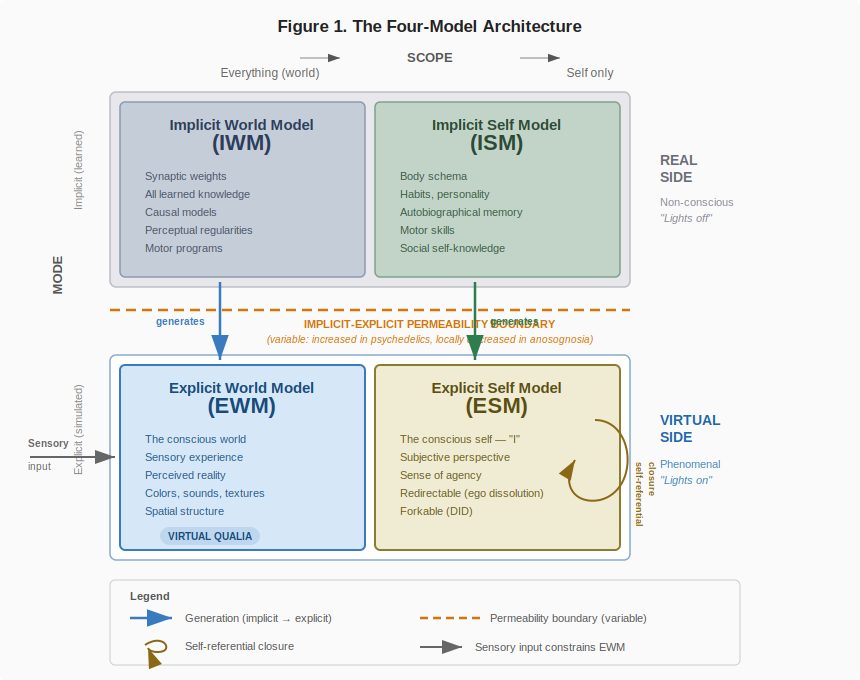
\includegraphics[width=0.85\textwidth]{figure1-four-model-architecture.png}
\caption{The four-model architecture. The two orthogonal axes---scope (world vs.\ self) and mode (implicit vs.\ explicit)---define four functionally distinct models. Implicit models (bottom) are substrate-level, learned, and non-conscious. Explicit models (top) are virtual, transient, and phenomenal.}
\label{fig:four-models}
\end{figure}

\textbf{The Implicit World Model (IWM)} encompasses the substrate's total accumulated knowledge about the world, stored in synaptic weights (or their functional equivalent in non-biological substrates). It includes everything the system has ever learned: perceptual regularities, causal models, spatial relationships, semantic knowledge, motor programs for interacting with the world. The IWM is never directly conscious. It operates ``in the dark''---providing the knowledge base from which the conscious simulation is generated, but never itself appearing in experience.

\textbf{The Implicit Self Model (ISM)} is the substrate's accumulated self-knowledge: body schema, proprioceptive calibration, motor skills, habits, personality traits, autobiographical memory structures, and social self-knowledge. Like the IWM, the ISM is never directly conscious. There is no unified homunculus---no inner observer reading the ISM. The ISM is a structural feature of the substrate, not an experiential one.

\textbf{The Explicit World Model (EWM)} is the conscious world---the real-time simulation of reality that constitutes perceptual experience. When you see a room, hear a voice, feel the texture of a surface, you are experiencing the EWM. It is generated from the IWM (which provides the world-knowledge) and current sensory input (which constrains and updates the simulation), but it is not identical to either. The EWM is a virtual construct---a transient pattern of activity, not a permanent structure.

\textbf{The Explicit Self Model (ESM)} is the conscious self---the real-time simulation of ``I'' that constitutes self-experience. It is the sense of being a subject, having a perspective, occupying a body, possessing a history, and being the author of one's actions. The ESM is generated from the ISM (which provides the self-knowledge) and current interoceptive and proprioceptive input, but like the EWM, it is virtual: a transient process, not a permanent entity.

\subsection{The Real/Virtual Split}

The four models divide into two fundamental categories:

\textbf{The real side} (IWM + ISM): These are physical, structural, learned, and non-conscious. They are stored in the substrate's architecture---in biological brains, primarily in synaptic weights, dendritic morphology, and connectivity patterns. They accumulate over the organism's lifetime through learning. They have no phenomenal character. ``Lights off.''

\textbf{The virtual side} (EWM + ESM): These are simulated, transient, generated, and phenomenal. They are patterns of activity---in biological brains, transient electrochemical dynamics. They are constructed in real time from the implicit models and current sensory input. They \textit{are} experience. ``Lights on.''

This division is the foundation of the theory's treatment of the Hard Problem (Section~3.4) and structures its account of every phenomenon it addresses.

\begin{figure}[htbp]
\centering
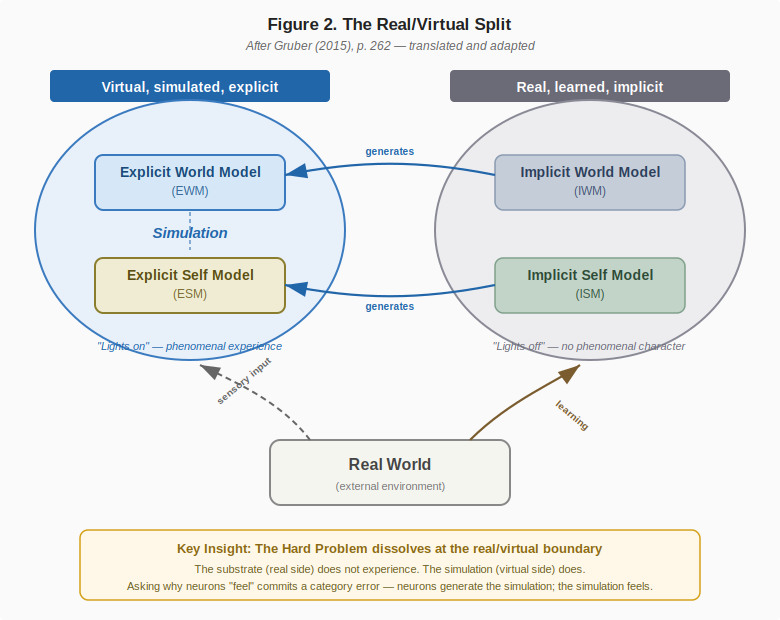
\includegraphics[width=0.85\textwidth]{figure2-real-virtual-split.png}
\caption{The ontological split between the real substrate (physical, structural, non-conscious---``lights off'') and the virtual phenomenal world (simulated, transient, experiential---``lights on''). Qualia exist only on the virtual side.}
\label{fig:real-virtual}
\end{figure}

The virtual models possess \textbf{software-like properties} that follow from their nature as simulations rather than structures:

\begin{itemize}
\item \textbf{They can be forked}: A single substrate can run multiple configurations of the ESM (see Section~6.2 on dissociative identity disorder).
\item \textbf{They can be cloned}: Physical separation of the substrate produces degraded but complete copies of the virtual models (see Section~6.4 on split-brain).
\item \textbf{They can be redirected}: The ESM requires input; disrupt normal self-referential input and it latches onto whatever input dominates (see Section~6.1 on psychedelics).
\item \textbf{They can be reconfigured}: Therapeutic interventions (CBT, exposure therapy) work by modifying the virtual models through substrate-level rewiring (see Section~6.6).
\end{itemize}

\subsection{Virtual Qualia: Dissolving the Hard Problem}

The central claim of the Four-Model Theory is that \textbf{qualia are virtual}. They are the way the simulated self (ESM) perceives its own states and the simulated world (EWM). Qualia exist within and are constitutive of the simulation; they do not exist at the substrate level.

This dissolves the Hard Problem by revealing a category error in its formulation:

\textbf{The standard formulation}: ``Why does physical processing (neuronal firing, synaptic transmission) feel like something?''

\textbf{The dissolution}: The physical processing \textit{does not} feel like anything. The IWM and ISM---the substrate-level implicit models---operate without any phenomenal character whatsoever. There is nothing it is like to be a synaptic weight. The simulation, however, \textit{does} feel---and within the simulation, qualia are simply what self-perception produces. Asking why neuronal firing feels like something is analogous to asking why transistor switching feels like running a video game. The transistors do not run the game at the level of individual switching; the virtual machine does. The neurons do not experience redness at the level of individual firing; the simulation does, and within the simulation, ``redness'' is simply the ESM's mode of registering a particular class of EWM content.

\textbf{Why self-simulation specifically?} A critic might object that this merely relocates the Hard Problem: why does \textit{this} virtual process have experience when a weather simulation does not? The answer lies in \textbf{self-referential closure}. A weather simulation models weather; it does not model \textit{itself modeling weather}. The four-model architecture creates a closed loop: the ESM is the system modeling its own modeling process. In this loop, the distinction between the model and the modeled collapses---the simulation \textit{is} the thing being simulated. Qualia are not an \textit{addition} to the self-modeling; they are the self-modeling as encountered from the inside of the loop. A non-self-referential simulation has an outside from which it can be described without remainder; a self-referential simulation at criticality has no such outside. The simulation \textit{is} its own observer, and observation-from-inside is what we call experience.

This is not a proof that self-referential simulation must be conscious---it is an argument that self-referential simulation is the \textit{kind} of process for which the Hard Problem's assumptions break down. Self-referential closure is precisely the condition under which the gap between process and feeling does not exist.

This is \textbf{not} illusionism in the sense of \citet{Dennett1991} or \citet{Frankish2016,Frankish2024}. Illusionism holds that qualia as traditionally conceived are illusions---there is nothing it is like, and our sense that there is something it is like is itself a misrepresentation. The Four-Model Theory holds that qualia are \textit{real within the simulation}. Within the EWM/ESM, experience has genuine phenomenal character. What is illusory is the assumption that this phenomenal character must be a property of the physical substrate. It is not. It is a property of the virtual process that the substrate runs.

This constitutes a \textbf{two-level ontology}: the substrate level (real side) has no experience, and the simulation level (virtual side) has genuine experience. Both levels are physical---the simulation is a physical process, not a supernatural one---but they have different ontological properties. The category error in the Hard Problem consists in conflating the two levels: seeking phenomenal properties at the substrate level where they do not exist.

The Explanatory Gap closes simultaneously. The gap between ``neurons fire in pattern X'' and ``I experience red'' is not a gap in our knowledge but a reflection of the level distinction. The neural firing pattern generates and sustains the simulation in which redness is experienced, but the firing pattern itself is not red and does not experience redness, just as a CPU's electrical states are not ``a spreadsheet'' even though they generate and sustain one.

\subsection{Graduated Levels of Consciousness}

Consciousness in the Four-Model Theory is not binary but graduated. The theory identifies a hierarchy of levels based on the depth of recursive self-modeling:

\textbf{Basic consciousness}: Minimal self-simulation. The system generates an EWM and a rudimentary ESM---it experiences a world and has a minimal sense of being a subject within it. This is the entry level: phenomenal experience exists but self-awareness is thin.

\textbf{Simply extended consciousness}: First-order self-observation. The system models itself---the ESM includes a model of the system's own states and processes. The organism not only experiences but is aware that it experiences.

\textbf{Doubly extended consciousness}: Second-order self-observation. The system models itself modeling itself. This enables reflection, metacognition, and the sense of being an observer of one's own mental processes.

\textbf{Triply extended consciousness}: Third-order self-observation. The system models itself modeling itself modeling itself. This supports the deepest forms of self-awareness, philosophical reflection, and the very intuition that consciousness is mysterious (connecting to the Meta-Problem---see Section~3.8). Notably, triply extended consciousness is also a prerequisite for the scientific study of consciousness itself: only a system capable of modeling its own modeling of its own experience can formulate the question ``What is consciousness?''

Each level corresponds to an additional layer of recursive self-modeling. The levels are not discrete stages but points along a continuum. Different organisms---and potentially different artificial systems---occupy different positions along this continuum, and individual organisms may fluctuate between levels depending on state (waking, dreaming, meditative, intoxicated).

\subsection{The Implicit--Explicit Boundary}

A key mechanism in the Four-Model Theory is the \textbf{permeability of the boundary between implicit models (IWM/ISM) and explicit models (EWM/ESM)}. Information becomes conscious when it is transferred from the implicit to the explicit side---when substrate-level knowledge or self-knowledge is incorporated into the running simulation.

In normal waking states, this boundary is \textbf{selectively permeable}: relevant information passes through based on attentional and contextual gating. You are not conscious of everything your IWM knows about the world or everything your ISM knows about yourself; you are conscious of what the current simulation requires.

The permeability of this boundary is variable, and its variation explains a wide range of phenomena (detailed in Section~6):

\begin{itemize}
\item \textbf{Psychedelic states}: Global increase in permeability---intermediate processing stages (normally implicit) become accessible to the explicit models. This explains the characteristic visual progression from simple phosphenes (V1-level) through geometric patterns (V2/V3-level) to complex imagery (higher visual areas) and eventually full dream-like scenes \citep{CarhartHarris2014}.
\item \textbf{Anosognosia}: Local decrease in permeability---the ISM contains the information (e.g., that a limb is paralyzed), but the transfer to the EWM is blocked for that specific domain.
\item \textbf{Pre-sleep/deep relaxation}: Gradually increasing permeability, producing the same bottom-up visual progression as psychedelics (phosphenes $\to$ geometrics $\to$ hypnagogic imagery).
\item \textbf{Meditation}: Trained modulation of permeability, enabling selective access to normally implicit processes.
\end{itemize}

\subsection{The Criticality Requirement}

The Four-Model Theory imposes a \textbf{physical prerequisite} for consciousness: the substrate must operate at or near the edge of chaos---Wolfram's Class~4 computational regime \citep{Wolfram2002}.

Wolfram classified cellular automata (and by extension computational systems generally) into four classes:
\begin{itemize}
\item \textbf{Class 1}: Converges to a fixed state. Too simple for consciousness.
\item \textbf{Class 2}: Periodic/repetitive. Too simple for consciousness.
\item \textbf{Class 3}: Chaotic/random. Too disordered for coherent consciousness.
\item \textbf{Class 4}: Complex/edge of chaos. Capable of universal computation. The regime in which consciousness can emerge.
\end{itemize}

This classification was applied to the question of consciousness in \citet{Gruber2015}, where it was argued that consciousness requires Class~4 dynamics---complex enough to sustain a self-simulation, ordered enough for that simulation to be coherent. This requirement was derived \textit{theoretically}, from the computational properties needed for real-time self-modeling, not from empirical neuroscience.

Independently, empirical neuroscience has converged on the same conclusion through a different path. \citet{Beggs2003} demonstrated neuronal avalanches consistent with self-organized criticality in cortical tissue. \citet{CarhartHarris2014} proposed the Entropic Brain Hypothesis, linking consciousness level to neural entropy. \citet{Tagliazucchi2012,Tagliazucchi2016} showed criticality signatures in waking fMRI and under LSD. \citet{Priesemann2013,Priesemann2014} characterized brain dynamics as slightly subcritical in normal waking states. This line of research was formally consolidated in the Consciousness and Criticality (ConCrit) framework \citep{AlgomShriki2026}, which synthesized evidence across multiple paradigms to establish that consciousness tracks criticality across pharmacological, pathological, and physiological state changes. A complementary meta-analysis of 140 datasets confirmed criticality as a unified setpoint of brain function \citep{HengenShew2025}.

\begin{table}[htbp]
\centering
\caption{Independent Convergence on Criticality}
\label{tab:criticality-convergence}
\begin{tabular}{lll}
\toprule
\textbf{Year} & \textbf{Development} & \textbf{Path} \\
\midrule
2002 & Wolfram publishes \textit{A New Kind of Science} & Computational theory \\
2003 & Beggs \& Plenz---neuronal avalanches & Empirical neuroscience \\
2014 & Carhart-Harris---Entropic Brain Hypothesis & Empirical neuroscience \\
\textbf{2015} & \textbf{Gruber---Class~4 / edge of chaos requirement} & \textbf{Theoretical (via Wolfram)} \\
2016 & Tagliazucchi et al.---LSD and criticality & Empirical neuroscience \\
2022 & ``Self-organized criticality as a framework'' (review) & Empirical neuroscience \\
2025 & Hengen \& Shew---meta-analysis of 140 datasets & Empirical neuroscience \\
\textbf{2025--26} & \textbf{ConCrit framework (Algom \& Shriki)} & \textbf{Theoretical/empirical synthesis} \\
\bottomrule
\end{tabular}
\end{table}

\begin{figure}[htbp]
\centering
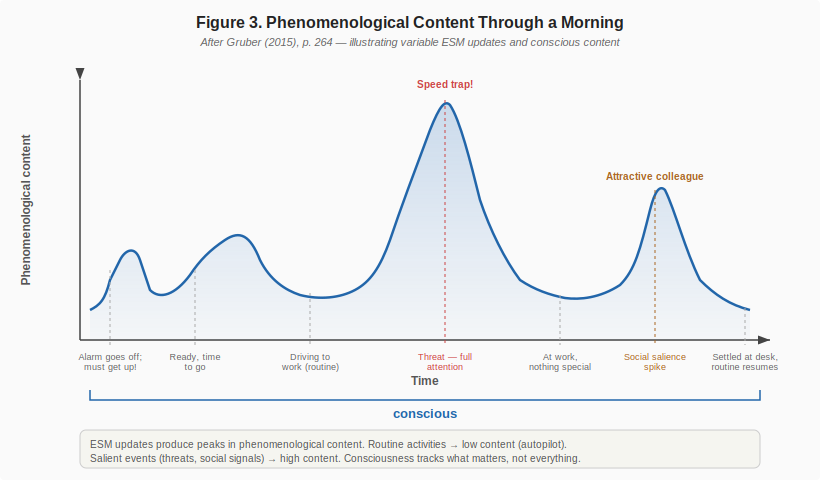
\includegraphics[width=0.85\textwidth]{figure3-phenomenological-content.png}
\caption{The structure of phenomenological content: what appears in the virtual world (EWM) and how the virtual self (ESM) experiences it. The boundary between implicit and explicit determines what reaches conscious awareness.}
\label{fig:phenomenological}
\end{figure}

Two independent paths---theoretical reasoning from computational first principles \citep{Gruber2015} and large-scale empirical neuroscience \citep{HengenShew2025,AlgomShriki2026}---converging on the same claim a decade apart. This convergence does not prove the Four-Model Theory correct, but it provides substantial independent support for one of its core predictions.

The Four-Model Theory distinguishes two thresholds for consciousness:
\begin{itemize}
\item \textbf{Physical threshold}: Criticality. The substrate must operate at Class~4 dynamics. Below this, no consciousness is possible regardless of architecture.
\item \textbf{Functional threshold}: Four-model architecture. The substrate must implement the four-model self-simulation. Above criticality but without the architecture, there is complex dynamics but no consciousness.
\end{itemize}

Both thresholds must be met. Criticality is necessary but not sufficient; the four-model architecture is necessary but not sufficient. Together they are sufficient.

\subsection{The Meta-Problem Dissolved}

The Meta-Problem---why we think there is a Hard Problem---receives a natural account within the Four-Model Theory. The ISM (Implicit Self Model) is \textbf{structurally inaccessible} to the ESM (Explicit Self Model). The conscious self cannot directly observe its own substrate. When the ESM attempts to model the basis of its own experience, it encounters a principled opacity: the implicit models that generate the simulation are not themselves part of the simulation.

This is why consciousness \textit{seems} mysterious. The ESM can represent that it is having an experience, but it cannot represent the mechanism by which the experience is generated---because that mechanism operates at the implicit/substrate level, which is by definition outside the explicit/virtual level. The result is the persistent intuition that something is being ``left out'' of any physical explanation: the ESM cannot find the mechanism within its own simulation, so it concludes the mechanism must be non-physical or fundamentally inexplicable.

This account shares features with Graziano's AST explanation---both invoke the self-model's necessary incompleteness---but grounds it in a more specific architecture (four models, real/virtual split) and connects it to the broader dissolution of the Hard Problem rather than treating the Meta-Problem in isolation.

%=============================================================================
\section{Philosophical Commitments}
%=============================================================================

The Four-Model Theory entails specific philosophical positions that were established through structured adversarial analysis and are internally consistent. This section develops and defends each commitment.

\subsection{Process Physicalism}

The theory is physicalist: both the substrate (implicit models) and the simulation (explicit models) are physical processes. There is no non-physical substance, no fundamental experiential property, no panpsychist micro-experience. Qualia are higher-order physical patterns---specifically, they are patterns of activity within the simulation that constitute the ESM's self-perception within the EWM.

This is process physicalism rather than identity theory: consciousness is not identical to any particular neural state but is constituted by the \textit{process} of self-simulation. The same conscious state could, in principle, be realized by different physical substrates---what matters is the functional architecture (four models at criticality), not the specific material.

Process physicalism avoids the difficulties of both type-identity theory (which struggles with multiple realization) and functionalism as traditionally conceived (which struggles with the Hard Problem). The Four-Model Theory adds the real/virtual level distinction to standard functionalism, which is what allows it to address phenomenality: qualia are not just functional roles but virtual properties of the simulation. They are real \textit{as virtual properties}---genuinely experiential but not properties of the substrate.

\subsection{Epiphenomenalism}

The theory commits to epiphenomenalism: consciousness---the phenomenal experience constituted by the virtual models---\textbf{observes but does not cause}. The substrate-level architecture (IWM, ISM, and the mechanisms that generate and maintain EWM and ESM) is causally efficacious: it processes information, makes decisions, generates behavior. The experience that accompanies this processing is a product of the architecture but does not feed back to influence the architecture's operation.

This entails that \textbf{free will is an illusion}: the ESM narrates and claims ownership of decisions that have already been made at the substrate level. The feeling of deciding is part of the simulation---a real experience within the virtual process---but it is not the cause of the behavior it seems to authorize. However, this illusion has a self-reinforcing quality: the very act of reflecting on free will---a triply extended operation in which the ESM examines its own decision-making model---can itself alter the substrate's future decision landscape, creating something functionally close to the libertarian ideal without requiring top-down phenomenal causation. This is consistent with Libet's \citeyearpar{Libet1985} readiness potential findings and their reinterpretation by \citet{Schurger2012}, and with Wegner's \citeyearpar{Wegner2002} analysis of the illusion of conscious will.

\textbf{Anticipated objection: If consciousness is epiphenomenal, why does it exist?}

The \textit{architecture} is selected for, not the \textit{experience}. The four-model self-simulation provides enormous adaptive advantages---predictive modeling, counterfactual reasoning, social cognition. Natural selection selects for these functional capabilities. Consciousness---the phenomenal experience that accompanies the self-simulation---is a necessary accompaniment of the architecture, not a separate feature that evolution selected for or against.

This framing avoids the strongest anti-epiphenomenalist arguments. \textbf{The zombie argument} \citep{Chalmers1996}: In the Four-Model Theory, zombies are not possible. The virtual models are not \textit{additions} to the substrate's activity---they \textit{are} the substrate's activity described at the virtual level. A system running the four-model architecture at criticality necessarily instantiates the self-referential simulation, just as a vortex in water is not added to the water's movement but is a description of it. \textbf{The knowledge argument} \citep{Jackson1982}: Mary gains acquaintance with a virtual quale---a property of the simulation she could not access from third-person substrate descriptions. This is consistent with epiphenomenalism: the new knowledge is real but does not require consciousness to have causal power. \textbf{The evolutionary argument}: The architecture is selected for; consciousness comes along necessarily.

\textbf{Quantum measurement}: As an entailment of epiphenomenalism, consciousness plays no role in quantum measurement or wavefunction collapse. Observer-dependent interpretations of quantum mechanics \citep{vonNeumann1932,Wigner1961} are rejected. This is consistent with the dominant position in contemporary physics (decoherence approaches; \citealp{Zurek2003}) and with the theory's commitment to physicalism.

\subsection{Weak Emergence}

Consciousness, in this theory, is weakly emergent: it is deducible in principle from a complete description of the substrate, even if it is practically irreducible due to the complexity of the system. There is no strong emergence, no magical threshold, no point at which ``something extra'' appears that could not have been predicted from the underlying physics.

This avoids the difficulties of both strong emergence (which is either mysterious or incoherent; \citealp{Kim1993}) and the panpsychist combination problem (which is unresolved; \citealp{Chalmers2016}). Consciousness does not arise from combining micro-experiences (there are none to combine) and does not require a special emergence law (there is none). It arises from the computational properties of a system running a self-simulation at criticality, just as a weather pattern arises from the thermodynamic properties of an atmosphere---no extra ingredient needed.

\subsection{Substrate Independence}

The six-layer mammalian neocortex is an evolutionary implementation of the four-model architecture, not a requirement for it. Consciousness is substrate-independent: any physical system capable of implementing the four-model architecture at criticality should produce consciousness.

Biological evidence already supports this. Corvids (crows, ravens) and parrots demonstrate cognitive abilities---tool use, planning, mirror self-recognition, social cognition---that strongly suggest consciousness, yet their brains have no neocortex. Their pallium is organized in nuclear clusters rather than layers \citep{Gunturkun2016}. Cephalopods (octopuses) demonstrate problem-solving and behavioral flexibility with an even more radically different brain architecture. If the Four-Model Theory is correct, these animals are conscious not because they share our neural architecture but because they have evolved functionally equivalent self-simulation architectures on different substrates---exactly what substrate independence predicts.

The implication for artificial consciousness is direct: a synthetic system implementing the four-model architecture at criticality should produce genuine consciousness. Current AI systems, including large language models, do not meet this specification. LLMs lack an Explicit Self Model (they do not run a real-time self-simulation), lack criticality (transformer inference is a feedforward pass---Class~1/2 dynamics), and lack the real/virtual split that grounds phenomenality. The theory predicts that the qualitative difference between interacting with a genuinely conscious artificial system and interacting with an LLM would be immediately and qualitatively distinguishable.

%=============================================================================
\section{Binding, Criticality, and Holographic Storage}
%=============================================================================

\subsection{Binding as an Emergent Property of Critical Dynamics}

The Four-Model Theory does not treat binding as a separate mechanism requiring a dedicated solution. Instead, binding is an emergent property of a substrate operating at criticality.

At the edge of chaos, the system exhibits maximal correlation length: distant parts of the substrate influence each other, local perturbations propagate globally, and information is integrated across the entire network. These are precisely the conditions under which distributed representations---features encoded across the full network rather than localized in specific neurons---are sustained and coordinated. Binding is not something the brain does \textit{in addition to} its other computations; it is a consequence of the dynamical regime in which the brain operates.

This is consistent with empirical findings. Gamma-band synchrony \citep{Gray1989,Rodriguez1999,Fries2005,Fries2015}, long-range thalamocortical coherence \citep{Llinas1993,Llinas1998}, and criticality signatures in neural dynamics \citep{Beggs2003,Tagliazucchi2012} all point toward the same conclusion: the unified character of conscious experience reflects the dynamical integration of a system operating at or near criticality, not a dedicated binding mechanism.

\subsection{Holographic Storage}

The implicit models (IWM and ISM) store information in a distributed, non-local manner across the substrate. This is a standard property of neural networks, well-characterized in the computational literature as distributed representations \citep{Hinton1986}, graceful degradation (loss of connections degrades but does not destroy stored information), and attractor dynamics (the network settles into basins of attraction that represent stored knowledge).

The term ``holographic'' is used here as an analogy, not a claim about optical holography: just as cutting a hologram in half produces two complete but lower-resolution images, splitting a neural network produces two degraded but functionally complete copies of the stored information. This property is critical for understanding split-brain phenomena (Section~6.4).

\subsection{Consciousness States Derived from Criticality}

The criticality requirement provides a unified account of when consciousness is present and when it is absent. Consciousness tracks the substrate's position relative to the critical point:

\begin{table}[htbp]
\centering
\caption{Consciousness States and Criticality}
\label{tab:consciousness-states}
\small
\begin{tabularx}{\textwidth}{lllXl}
\toprule
\textbf{State} & \textbf{Criticality} & \textbf{Four-model status} & \textbf{Consciousness prediction} & \textbf{Key evidence} \\
\midrule
Normal waking & At/near critical & All four active & Full consciousness & High PCI \\
REM sleep & Near-critical & EWM/ESM on internal input & Degraded (dream) & Moderate PCI \\
Deep NREM & Subcritical & EWM/ESM collapse & Absent & Low PCI \\
Propofol & Forced subcritical & EWM/ESM suppressed & Absent & PCI $\approx$ 0 \\
Ketamine & NOT subcritical & EWM/ESM on wrong input & Present but disconnected & Increased entropy \\
Psychedelics & At/past critical & All active, permeability $\uparrow$ & Present, altered & Enhanced complexity \\
Vegetative state & Typically subcritical & EWM/ESM collapsed & Absent (usually) & Low metabolism \\
Covert awareness & At criticality & EWM/ESM intact, output damaged & Present but unexpressible & Owen et al. \\
MCS & Fluctuating & Intermittent EWM/ESM & Intermittent & Fluctuating PCI \\
\bottomrule
\end{tabularx}
\end{table}

The key distinction highlighted by this framework is between \textbf{propofol} and \textbf{ketamine}. Both are anesthetics, yet their phenomenology differs dramatically. Propofol produces absence: patients report no experience during propofol anesthesia \citep{Alkire2000,Boly2012}. Ketamine produces the ``K-hole''---vivid, often bizarre experiences of dissociation, out-of-body phenomena, and altered identity \citep{Corlett2013}. The Four-Model Theory predicts this difference: propofol pushes the substrate subcritical (disrupting thalamocortical connectivity, suppressing complexity), abolishing the conditions for consciousness. Ketamine does \textit{not} push the substrate subcritical---it increases neural entropy \citep{Schartner2015}---but disrupts normal sensory input processing, causing the EWM and ESM to operate on internal and distorted signals. Consciousness is present but disconnected from external reality.

This is a genuine explanatory advantage. Most theories struggle to account for why two agents classified as ``anesthetics'' produce such radically different phenomenological profiles. The criticality framework makes the distinction natural: what matters is not the pharmacological classification but the effect on the substrate's dynamical regime.

%=============================================================================
\section{Explanatory Range}
%=============================================================================

A theory's value lies partly in its ability to derive diverse phenomena from a small set of principles. The Four-Model Theory's five principles---criticality, virtual qualia, redirectable ESM, variable implicit--explicit permeability, and virtual model forking---generate accounts of phenomena across psychopharmacology, clinical neurology, sleep science, comparative cognition, and clinical psychology. This section demonstrates that range.

\subsection{Psychedelic Phenomenology}

Psychedelic substances (LSD, psilocybin, DMT, mescaline) produce a characteristic phenomenological profile: visual intensification and distortion, synesthesia, altered time perception, enhanced pattern recognition, emotional intensification, ego dissolution at high doses, and---with certain compounds and doses---radical identity alteration including the experience of ``becoming'' non-self entities \citep{CarhartHarris2012,CarhartHarris2016,Timmermann2019,Timmermann2023}.

The Four-Model Theory accounts for this profile through three mechanisms:

\textbf{Implicit--explicit permeability increase.} Psychedelics increase the global permeability of the boundary between implicit and explicit models. Intermediate processing stages---normally implicit and inaccessible---leak through to the simulation. This produces the characteristic visual progression:

\begin{itemize}
\item \textbf{Low dose / early onset}: V1-level processing becomes accessible $\to$ simple phosphenes, enhanced contrast, breathing/movement in static patterns.
\item \textbf{Increasing dose}: V2/V3-level processing becomes accessible $\to$ geometric patterns, fractals, tessellations (form constants; \citealp{Kluver1966}).
\item \textbf{Higher dose}: Higher visual area processing becomes accessible $\to$ faces, figures, scenes.
\item \textbf{Very high dose}: Full intermediate processing accessible $\to$ complex dream-like visions, narrative sequences.
\end{itemize}

This progression is not random. It follows the visual processing hierarchy in a predictable, dose-dependent order. The Four-Model Theory predicts this ordered progression as a direct consequence of the permeability gradient: lower-level (earlier, simpler) processing stages become accessible before higher-level (later, more complex) ones, because the permeability increase propagates up the hierarchy.

\textbf{Ego dissolution = ESM redirection, not ESM abolition.} At high doses, psychedelics disrupt the normal self-referential input to the ESM. The ESM does not cease to exist---it continues to run---but it loses its normal input and latches onto whatever dominates the available input stream. This produces the experience of ego dissolution: the feeling that the boundary between self and world has dissolved, that one's identity has merged with the environment or with abstract patterns.

Critically, this mechanism predicts that the \textit{content} of ego dissolution is not random but is determined by the dominant input available to the ESM. This is dramatically confirmed by the phenomenology of \textbf{salvia divinorum} (Salvinorin~A). Salvia users reliably report experiences of ``becoming'' objects or entities in their immediate environment: becoming a piece of furniture, becoming a wall, becoming a character from a television show playing in the room, becoming a geometric pattern. The Four-Model Theory predicts exactly this: the ESM, deprived of normal self-input, latches onto whatever sensory input dominates---visual input from the room, auditory input from media, proprioceptive input from the body's contact surfaces. The identity experience tracks the dominant input in a dose-dependent, input-dependent, and therefore \textit{predictable} manner.

No competing theory of consciousness can generate this prediction. IIT, GNW, HOT, PP, and AST have no mechanism for identity content tracking during ego dissolution. This is arguably the theory's most distinctive prediction (see Section~8, Prediction~3).

\textbf{Intensity as novelty.} Psychedelic profundity reflects not increased consciousness \textit{level} but increased \textit{novel content}. The permeability increase floods the simulation with normally implicit information. This is experienced as radically novel because the conscious self has never encountered this content, even though the substrate has been processing it all along.

\subsection{Anesthesia and Clinical Disorders}

\textbf{Propofol anesthesia}: Pushes the substrate subcritical $\to$ the conditions for consciousness are abolished $\to$ the simulation collapses $\to$ no experience. (See Table~\ref{tab:consciousness-states}.)

\textbf{Ketamine}: Does not push subcritical; increases entropy $\to$ consciousness persists but on distorted/internal input $\to$ dissociative experience, K-hole phenomenology.

\textbf{Vegetative state}: Substrate is typically subcritical $\to$ no consciousness. But the Four-Model Theory makes a nuanced prediction: if the substrate is at criticality but \textit{output pathways} are damaged (motor cortex, brainstem circuits), consciousness is present but unexpressible. This is precisely the phenomenon of \textbf{cognitive motor dissociation} (CMD), documented by \citet{Owen2006} and \citet{Monti2010}, in which patients clinically diagnosed as vegetative demonstrate awareness through brain-imaging paradigms. The theory predicts that the distinction between truly vegetative (subcritical substrate) and covertly conscious (critical substrate with damaged output) should be detectable via criticality measures such as PCI \citep{Casali2013,Casarotto2016}.

\textbf{Minimally conscious state}: The substrate fluctuates around the criticality threshold $\to$ intermittent consciousness, explaining the characteristic behavioral variability.

\textbf{Cotard's delusion}: Patients report believing they are dead, that their organs have disappeared, or that they do not exist. The Four-Model Theory derives this from the same mechanism as salvia: the ESM receives severely distorted interoceptive input (due to neurological damage or psychiatric disorder). Deprived of normal self-referential signals, the ESM constructs the best model it can from the available (distorted) input---and ``I am dead'' is the ESM's interpretation of the absence of normal embodied signals. This is the same redirectable-ESM mechanism that produces ``I am a chair'' under salvia, applied to a clinical context.

\textbf{Anosognosia}: Patients with anosognosia (typically following right-hemisphere stroke) are unaware of their own deficits---they deny being paralyzed, blind, or impaired, even in the face of clear evidence. The Four-Model Theory explains this as a \textbf{local decrease in implicit--explicit permeability}: the ISM contains the information about the deficit (the substrate registers the paralysis), but the transfer to the EWM is blocked for that specific domain. The patient's simulation simply does not include the deficit, so the patient genuinely does not experience it.

This is the \textbf{inverse} of the psychedelic mechanism: psychedelics globally increase permeability (making the implicit accessible), while anosognosia locally decreases permeability (making a specific aspect of the implicit inaccessible). The Four-Model Theory connects these phenomena under a single principle---variable permeability---and generates a cross-domain prediction: psychedelics should alleviate anosognosia by compensating for the local block with a global permeability increase (see Section~8, Prediction~4).

\textbf{Dissociative Identity Disorder (DID)}: The virtual models, being software-like, can be \textbf{forked}. DID represents a substrate running multiple ESM configurations---multiple self-models---that alternate in controlling the simulation. Each alter is a distinct configuration of the ESM, with its own self-narrative, emotional profile, and behavioral patterns, running on the same substrate. This is not a metaphor: the theory predicts that distinct alters should correspond to distinct patterns of neural activity, detectable with neuroimaging (see Section~8, Prediction~9).

\subsection{Dreams}

Dreaming represents the simulation running in \textbf{degraded mode}: near-critical dynamics (sufficient for consciousness) but with external input cut off (sensory deprivation during sleep).

The EWM continues to generate a world---but without the constraint of sensory input, the simulation draws on the IWM's stored knowledge, producing the characteristic features of dreams: familiar places and people, impossible physics, narrative incoherence, and emotional intensity. The ESM continues to generate a self---you experience dreams as happening to ``you''---but with reduced metacognitive oversight, producing the characteristic lack of insight in dreams (you accept impossible events without question).

\textbf{Lucid dreaming} provides direct evidence for the software-like quality of the virtual models. In a lucid dream, the dreamer becomes aware that they are dreaming: the ESM ``toggles on'' more fully, gaining metacognitive access within the dream state. The Four-Model Theory predicts that lucid dream onset corresponds to a \textbf{criticality threshold crossing}---a step-like increase in neural complexity as the ESM activates more fully. This should be detectable as a discontinuity in EEG complexity measures at the moment of lucid dream onset (see Section~8, Prediction~8).

The criticality framework also explains the \textbf{NREM/REM transition}: as the brain's dynamical state fluctuates during sleep, crossing the criticality threshold produces the transition from non-conscious deep sleep to conscious dreaming. The 90-minute ultradian cycle corresponds to an oscillation of the substrate around the critical point.

\subsection{Split-Brain}

Callosotomy produces the classic split-brain syndrome \citep{Gazzaniga1962,Gazzaniga2000}. The Four-Model Theory offers a more precise account than the traditional ``two minds in one brain.''

Because the implicit models store information holographically (Section~5.2), physical separation does not cleanly divide the models into left and right halves. Instead, it produces \textbf{two degraded but functionally complete copies}. Each hemisphere retains a degraded version of the IWM, ISM, EWM, and ESM---complete enough to sustain consciousness but lacking the resolution and scope of the intact system.

This accounts for the key features of split-brain behavior:
\begin{itemize}
\item \textbf{Each hemisphere sustains independent consciousness}: Both are above the criticality threshold and both have complete (if degraded) four-model architectures.
\item \textbf{The left hemisphere interpreter} \citep{Gazzaniga2000}: The left hemisphere's ESM confabulates explanations for behavior initiated by the right hemisphere. This is the \textit{same confabulation mechanism} observed in Cotard's delusion, anosognosia, and salvia experiences: an ESM constructing the best narrative it can from incomplete input.
\item \textbf{Degradation rather than clean division}: Split-brain patients do not show perfectly hemispheric specialization; they show graded deficits \citep{Pinto2017}, consistent with holographic degradation rather than binary splitting.
\end{itemize}

\subsection{Animal Consciousness}

The theory's commitments---continuum (not binary), substrate independence, criticality threshold---predict a \textbf{gradient} of animal consciousness. Mammals implement the four-model architecture in graduated form, with even simple cortices (rodents) supporting basic consciousness---rudimentary simulation sufficient for phenomenal experience but thin in self-awareness.

\textbf{Corvids and parrots} present a crucial test case: tool manufacture, mirror self-recognition, social deception, and future planning---yet no neocortex, with pallium organized in nuclear clusters \citep{Gunturkun2016}. The theory predicts these animals are conscious because they have evolved functionally equivalent self-simulation architectures on a different substrate. \textbf{Cephalopods} extend this logic further, with largely decentralized nervous systems that should produce consciousness with unusual features. Both cases test substrate independence directly.

\subsection{Clinical Psychology Bridge}

The virtual-model framework extends to clinical phenomena. \textbf{CBT} works as virtual model reprogramming: repeated corrective experience drives substrate-level rewiring (synaptic plasticity), modifying the ISM, which changes the ESM's self-model. \textbf{Phobias} are EWM misconfigurations where threat representation exceeds the IWM's evidence base; exposure therapy updates the IWM to correct the EWM.

\textbf{The placebo effect} is consistent with epiphenomenalism: placebo activates substrate-level expectation circuits (endogenous opioid release) that operate in parallel with---not caused by---the conscious experience of hope. The correlation between conscious expectation and physical effect is real but non-causal: both are products of the same substrate processes.

\textbf{Conversion disorder} is the inverse of blindsight: in blindsight, the substrate processes visual information without including it in the EWM; in conversion disorder, the EWM models a deficit (paralysis, blindness) that the intact substrate does not have.

%=============================================================================
\section{Comparative Analysis}
%=============================================================================

This section provides a systematic comparison between the Four-Model Theory and six major competitors across the eight requirements established in Section~2. The comparison aims to be fair: each theory's genuine strengths are acknowledged, and the Four-Model Theory's advantages are located precisely.

\subsection{Scoring Matrix}

Table~\ref{tab:comparison} presents an assessment of how each theory addresses the eight requirements. All ratings reflect the present author's judgment and are offered as a starting point for discussion, not as definitive verdicts. Readers are encouraged to consult the primary sources and form their own assessments. Where a theory's proponents would likely contest a rating, this is noted.

\textbf{Assessment criteria}: \textit{Addresses}~= the theory provides a substantive, defended account of this requirement. \textit{Partial}~= the theory provides a relevant account that leaves significant aspects unresolved. \textit{Minimal}~= the theory touches on this requirement but does not develop a full treatment. \textit{Silent}~= the theory does not address this requirement (which may reflect deliberate scope limitation rather than failure). \textit{N/A}~= the requirement does not apply given the theory's ontological commitments.

\begin{table}[htbp]
\centering
\caption{Theory Comparison Across Eight Requirements}
\label{tab:comparison}
\small
\begin{tabular}{lccccccc}
\toprule
\textbf{Requirement} & \textbf{Four-Model} & \textbf{IIT} & \textbf{GNW} & \textbf{HOT} & \textbf{PP} & \textbf{AST} & \textbf{RPT} \\
\midrule
Hard Problem & Addresses$^\dagger$ & Addresses$^\ddagger$ & Silent$^*$ & Partial & Silent$^*$ & Partial & Silent \\
Explanatory Gap & Addresses$^\dagger$ & Addresses$^\ddagger$ & Silent$^*$ & Partial & Silent$^*$ & Partial & Silent \\
Boundary & Addresses & Addresses & Partial & Minimal & Partial & Partial & Partial \\
Structure & Addresses & Addresses & Partial & Partial & Addresses & Partial & Partial \\
Binding & Addresses & Addresses & Partial & Minimal & Partial & Minimal & Partial \\
Combination & Addresses & Minimal$^\S$ & N/A & N/A & N/A & N/A & N/A \\
Causal Role & Addresses$^\|$ & Partial & Partial & Partial & Addresses & Partial & Addresses \\
Meta-Problem & Addresses & Minimal & Partial & Partial & Partial & Addresses & Minimal \\
\bottomrule
\end{tabular}

\smallskip
\raggedright\footnotesize
$^\dagger$~Dissolution via virtual qualia.
$^\ddagger$~Axiomatic identification of consciousness with $\Phi$; whether this constitutes a solution or a redefinition is debated.
$^\S$~IIT's panpsychist commitments lead to the Combination Problem \citep{Chalmers2016}, which remains unresolved.
$^*$~GNW and PP proponents argue these theories address the ``real problem'' of consciousness \citep{Seth2021}---explaining the structure and contents of experience---even if they do not address the Hard Problem as Chalmers defines it. This is a legitimate methodological choice; the ``Silent'' rating reflects the scope of the requirement as defined in Section~2, not a judgment on overall merit.
$^\|$~Epiphenomenal.
\end{table}

\subsection{Theory-by-Theory Comparison}

\textbf{Integrated Information Theory} (IIT; \citealp{Tononi2004}; \citealp{Albantakis2023}). IIT's strengths are mathematical rigor, its qualia space treatment of experiential structure, and a principled boundary via the exclusion postulate. However, its axiom-based identification of consciousness with $\Phi$ leads to panpsychist consequences, the Combination Problem remains unresolved \citep{Chalmers2016}, $\Phi$ is computationally intractable for realistic systems \citep{Aaronson2014}, and the unfolding argument \citep{Doerig2019} challenges its central claim about recurrence. The Four-Model Theory avoids panpsychism, has no combination problem (weak emergence), and generates predictions without computing $\Phi$.

\textbf{Global Neuronal Workspace} (GNW; \citealp{Baars1988}; \citealp{Dehaene2011}). GNW's empirically tractable broadcasting mechanism provides a clear account of access consciousness. However, it is silent on the Hard Problem---explaining \textit{when} but not \textit{why} broadcast produces experience. The COGITATE results \citep{COGITATE2025} were problematic: posterior cortex, not the frontoparietal workspace, showed the strongest consciousness-related activity. The Four-Model Theory agrees that broadcasting/integration is mechanistically important but adds the real/virtual distinction that addresses phenomenality.

\textbf{Higher-Order Theories} (HOT; \citealp{Rosenthal2005}; \citealp{Lau2011}). HOT naturally explains which states are conscious (those with higher-order representations) and partially addresses the Meta-Problem. However, it does not address binding, leaves the Hard Problem only partially treated (why does higher-order representation produce phenomenality?), and its boundary-setting is imprecise. The Four-Model Theory shares HOT's emphasis on self-representation but embeds it in the richer four-model architecture, explaining \textit{why} self-representation produces phenomenality through the virtual qualia framework.

\textbf{Predictive Processing} (PP; \citealp{Friston2010}; \citealp{Seth2021}). PP's integration with a broader theory of brain function and its strong accounts of experiential structure and causal role (via active inference) are genuine strengths. Seth's controlled hallucination framework is among the most empirically productive in the field. However, PP is explicitly silent on the Hard Problem \citep{Seth2021}. Markov blankets may also be too liberal for boundary-setting. The Four-Model Theory agrees that prediction is central but adds the four-model architecture, criticality requirement, and real/virtual distinction that PP lacks.

\textbf{Attention Schema Theory} (AST; \citealp{Graziano2013}). AST provides the strongest existing account of the Meta-Problem: the self-model of attention is necessarily incomplete, producing the intuition of mystery. However, AST is deflationary about phenomenality and does not address binding. The Four-Model Theory incorporates AST's Meta-Problem insight---the ESM's structural inaccessibility to its own substrate---but adds the virtual qualia framework that explains \textit{why} phenomenality exists, not just why we think it does.

\textbf{Recurrent Processing Theory} (RPT; \citealp{Lamme2006,Lamme2010}). RPT's empirical specificity and clear account of the causal role are strengths, with strong support from visual masking paradigms. However, it is silent on the Hard Problem and limited in scope to visual consciousness. The Four-Model Theory is compatible with RPT at the mechanistic level---recurrent processing likely implements the real-time simulation---but adds the architectural and philosophical specificity that RPT lacks.

\subsection{Emerging Frameworks (2024--2026)}

\textbf{Biological computationalism} \citep{Milinkovic2025} argues that consciousness requires specifically biological computation, challenging substrate independence. The Four-Model Theory treats substrate independence as an empirical prediction: artificial substrates implementing the four-model architecture at criticality should produce consciousness. The existence of conscious corvids with non-cortical brain architecture (nuclear pallium; \citealp{Gunturkun2016}) favors substrate independence.

The \textbf{Multiple Generator Hypothesis} \citep{KirkebyHinrup2025} proposes consciousness arises from multiple independent mechanisms. This is potentially compatible: the four models could be understood as distinct generators unified by the criticality requirement and implicit--explicit boundary mechanism.

\subsection{Summary of Comparative Advantages}

\begin{enumerate}
\item \textbf{Addressing the Hard Problem without panpsychism or strong emergence}: Virtual qualia dissolve the Hard Problem through a two-level ontology that remains fully physicalist.
\item \textbf{Unifying binding with criticality}: Binding is a consequence of critical dynamics, not a separate mechanism.
\item \textbf{The redirectable ESM}: Unique mechanism for identity-content determination during ego dissolution (Predictions~3 and~4).
\item \textbf{Connecting psychedelics and anosognosia}: Variable permeability links these phenomena under a single principle.
\item \textbf{The Meta-Problem as structural consequence}: The ESM's opacity to its own substrate explains the intuition of mystery.
\end{enumerate}

The theory's primary disadvantage is the absence of mathematical formalization. IIT's $\Phi$ formalism and PP's free energy mathematics provide quantitative precision that the Four-Model Theory currently lacks (see Section~9).

%=============================================================================
\section{Novel Testable Predictions}
%=============================================================================

A theory is only as valuable as the predictions it generates. The Four-Model Theory yields nine novel testable predictions, several of which are unique---no competing theory can generate them.

\subsection{Prediction 1: Distinct fMRI Signatures for Each Model}

\textbf{Statement}: If the four models are functionally distinct processes, tasks that selectively engage a single model should produce distinct, reproducible neural activation patterns detectable via fMRI. Specifically: IWM-dominant tasks (e.g., passive recognition of familiar stimuli, implicit priming) should activate different networks than ISM-dominant tasks (e.g., habitual motor sequences, implicit body-schema tasks), which should differ from EWM-dominant tasks (e.g., active perceptual discrimination, novel scene processing) and ESM-dominant tasks (e.g., self-reflection, agency judgments, mirror self-recognition).

\textbf{Mechanism}: The four models are functionally distinct processes (not spatially localized brain regions), but distinct processes should nonetheless recruit distinguishable distributed networks. The implicit models (IWM, ISM) should preferentially engage substrate-level storage networks (hippocampal--cortical for IWM, somatosensory--cerebellar for ISM), while the explicit models (EWM, ESM) should preferentially engage simulation networks (sensory cortices for EWM, default mode network and medial prefrontal cortex for ESM).

\textbf{Testability}: High. Design a factorial task battery crossing scope (world vs.\ self) with mode (implicit vs.\ explicit), yielding four conditions. Contrast activation maps across conditions using standard fMRI subtraction or multivariate pattern analysis. The prediction is a double dissociation: scope $\times$ mode interaction effects in distributed networks.

\textbf{Unique?}: Yes in the specific form. While individual contrasts (e.g., self vs.\ world processing) are well-studied, the Four-Model Theory predicts a specific $2\times2$ factorial structure in neural activation that no other theory mandates. This prediction is placed first because it most directly tests the four-model architecture itself---the central structural claim of the theory.

\subsection{Prediction 2: Psychedelic Content Maps the Processing Hierarchy}

\textbf{Statement}: Under psychedelics, visual content progresses through the cortical processing hierarchy in an ordered, dose-dependent sequence: V1-level content (phosphenes, enhanced contrast) $\to$ V2/V3-level content (geometric patterns, form constants) $\to$ higher visual area content (faces, figures) $\to$ complex scenes (dream-like narratives).

\textbf{Mechanism}: Increasing implicit--explicit permeability exposes intermediate processing stages in hierarchical order.

\textbf{Testability}: High. Combine graded dosing protocols with concurrent fMRI or MEG to track the spatial progression of activation, correlated with subjective report of content type. Partial evidence already exists \citep{CarhartHarris2016,Timmermann2023} but has not been systematically tested as an ordered, dose-correlated progression.

\textbf{Unique?}: Partially. PP also predicts hierarchical processing under psychedelics but does not predict the specific ordered content progression as a function of dose.

\subsection{Prediction 3: Ego Dissolution Content Is Controllable}

\textbf{Statement}: During psychedelic ego dissolution, the content of the altered identity experience (what the subject ``becomes'') tracks the dominant sensory input. By controlling the sensory environment during ego dissolution, the identity content can be predicted and directed.

\textbf{Mechanism}: The ESM, deprived of normal self-referential input, latches onto whatever input dominates the available stream. Control the input $\to$ control the identity content.

\textbf{Testability}: High. Administer ego-dissolution-inducing doses of psilocybin or salvia divinorum under controlled conditions. Vary the dominant sensory input (specific visual scenes, specific auditory environments, specific tactile inputs) across conditions. Measure correspondence between controlled input and reported identity content.

\textbf{Unique?}: \textbf{Yes---no competing theory can generate this prediction.} IIT, GNW, HOT, PP, and AST have no mechanism for specifying what a subject will ``become'' during ego dissolution. This is the theory's most distinctive empirical prediction.

\subsection{Prediction 4: Psychedelics Alleviate Anosognosia}

\textbf{Statement}: Administration of psychedelic substances at sub-ego-dissolution doses should alleviate anosognosia by globally increasing implicit--explicit permeability, compensating for the local permeability block that causes the deficit unawareness.

\textbf{Mechanism}: Anosognosia = local permeability block. Psychedelics = global permeability increase. The global increase should overwhelm the local block, allowing the deficit information in the ISM to reach the EWM.

\textbf{Testability}: Medium (requires clinical trial with stroke patients). Could begin with case studies or observational reports of psychedelic use by patients with anosognosia. Psilocybin-assisted therapy is already being tested for various neuropsychiatric conditions, providing a potential clinical pathway.

\textbf{Unique?}: \textbf{Yes---this is a cross-domain surprise prediction.} No other theory connects psychedelics and anosognosia through a single mechanism. Confirmation would be strong evidence for the variable-permeability principle.

\subsection{Prediction 5: All Anesthetics Converge on Criticality Disruption}

\textbf{Statement}: Despite diverse receptor-level mechanisms (GABAergic, NMDA, opioid, $\alpha_2$-adrenergic), all agents that abolish consciousness do so by pushing the substrate below the criticality threshold. Agents that alter but do not abolish consciousness (ketamine, low-dose psychedelics) do not push below criticality.

\textbf{Mechanism}: The criticality requirement is the physical threshold for consciousness; any mechanism that disrupts criticality disrupts consciousness, regardless of receptor pathway.

\textbf{Testability}: High. Measure criticality indicators (PCI, Lempel--Ziv complexity, power-law exponents, detrended fluctuation analysis) across the full range of anesthetic agents at equi-potent doses. The prediction is that abolition of consciousness always correlates with subcriticality, and preserved consciousness (even if altered) always correlates with maintained criticality.

\textbf{Unique?}: Shared with the ConCrit framework \citep{AlgomShriki2026} and the criticality meta-analysis \citep{HengenShew2025}. However, the Four-Model Theory predicted this from theoretical first principles \citep{Gruber2015}, prior to the empirical consolidation.

\subsection{Prediction 6: Split-Brain Produces Holographic Degradation}

\textbf{Statement}: After callosotomy, each hemisphere retains a degraded but functionally \textit{complete} set of cognitive and experiential capacities---not a clean hemispheric specialization. The degradation should be proportional to the extent of commissural severing (partial callosotomy $\to$ partial degradation).

\textbf{Mechanism}: Holographic storage. Information is distributed across the full substrate; cutting connections degrades both copies but does not destroy either.

\textbf{Testability}: High. Systematic cognitive assessment of split-brain patients across domains, testing for the predicted pattern of bilateral but degraded capabilities rather than clean lateralization. \citet{Pinto2017} provide preliminary evidence in this direction.

\textbf{Unique?}: Yes, in the specific form. Standard neuroscience acknowledges some bilateral capacity, but the Four-Model Theory provides the theoretical basis (holographic storage) and predicts the specific pattern (graded degradation proportional to disconnection, not binary split).

\subsection{Prediction 7: Criticality + Four Models = Consciousness in Artificial Substrates}

\textbf{Statement}: A synthetic system implementing the four-model architecture at criticality will exhibit consciousness. The qualitative difference between interacting with such a system and interacting with a current LLM will be immediately and qualitatively distinguishable.

\textbf{Mechanism}: Substrate independence. Consciousness depends on function (four models at criticality), not on material (biological neurons).

\textbf{Testability}: Medium (requires significant engineering development). However, intermediate tests are possible: systems with partial implementations (e.g., two models instead of four, or four models without criticality) should show partial consciousness indicators, detectable through behavioral signatures and neural/computational complexity measures.

\textbf{Unique?}: Yes in the specific form. Other theories (PP, GNW) are compatible with artificial consciousness but do not provide a specific architectural blueprint.

\subsection{Prediction 8: Lucid Dream Onset Is a Criticality Threshold Crossing}

\textbf{Statement}: The transition from non-lucid to lucid dreaming corresponds to a step-like increase in neural complexity, consistent with the substrate crossing a criticality threshold. This transition should be detectable as a discontinuity in EEG complexity measures, not a gradual change.

\textbf{Mechanism}: Lucid dreaming = ESM activation within the dream state. ESM activation requires sufficient criticality to support the additional level of self-modeling.

\textbf{Testability}: High. EEG/polysomnographic recording with concurrent signaling by lucid dreamers (established paradigm; \citealp{LaBerge1985}). Analyze complexity measures (PCI, Lempel--Ziv, spectral exponents) in a time-locked window around the signaled onset of lucidity. The prediction is a step-like increase, not a gradual ramp.

\textbf{Unique?}: Partially shared. Criticality frameworks in general would predict complexity changes during lucid dreaming, but the specific prediction of a step-like discontinuity (reflecting threshold-crossing rather than gradual increase) is distinctive.

\subsection{Prediction 9: DID Alters Have Distinct Neural Process Signatures}

\textbf{Statement}: Different alters in DID correspond to distinct, measurable configurations of neural activity---not merely behavioral differences or different self-reports, but different neural dynamics detectable through neuroimaging.

\textbf{Mechanism}: Virtual model forking. Each alter is a distinct configuration of the ESM, running on the same substrate but with different parameters. Different parameters should produce different activity patterns.

\textbf{Testability}: High. fMRI or EEG recording during controlled alter switching in DID patients. Compare within-patient across-alter variability against within-patient within-alter variability. The prediction is that across-alter variability will be significantly greater than within-alter variability and will show consistent alter-specific patterns.

\textbf{Unique?}: Yes. While some neuroimaging studies of DID exist \citep{Reinders2006,Reinders2014}, the Four-Model Theory provides the theoretical basis for predicting \textit{consistent, alter-specific neural signatures} rather than merely \textit{differences}. The theory predicts a specific organizational principle: each alter is a distinct ESM configuration, so the neural differences should be located in ESM-related networks (particularly default mode network / medial prefrontal / posterior cingulate regions).

\subsection{The Ultimate Prediction}

If the Four-Model Theory is correct, it should be possible to \textit{build} a conscious machine by implementing the specified architecture: four nested models (IWM, ISM, EWM, ESM) operating at criticality on a substrate of sufficient complexity. The theory predicts that such a system would not merely simulate consciousness (as an LLM might be said to do) but would \textit{be} conscious---would have genuine phenomenal experience constituted by its virtual models.

This prediction is not currently testable---the engineering does not yet exist, and even if it did, the other-minds problem would make verification philosophically difficult. However, the prediction sets a bold bar: if the theory is correct, the difference between interacting with a conscious artificial system and interacting with any current AI should be qualitatively obvious to human observers, just as the difference between a conversation with a conscious human and a conversation with a cleverly programmed chatbot is (according to the theory) a difference in \textit{kind}, not merely in degree.

%=============================================================================
\section{Open Questions}
%=============================================================================

Intellectual honesty requires identifying what the theory does not yet resolve. These are research frontiers, not theoretical weaknesses---they are questions that arise \textit{from} the theory and that the theory's framework helps to sharpen.

\textbf{1. Are all four models virtual?} The theory as presented describes the implicit models (IWM, ISM) as ``real side'' and the explicit models (EWM, ESM) as ``virtual side.'' But it is not certain that this division is sharp. The implicit models might themselves have virtual properties---they are, after all, \textit{models}, not raw physics. If the implicit models are also virtual in some sense, what constitutes the ``real side''? The raw physical substrate with no model-level description? This is an open question even for the theory's author, and its resolution may have consequences for the theory's treatment of the Hard Problem.

\textbf{2. Mathematical formalization.} The theory's criticality requirement is specified qualitatively (Wolfram's Class~4 regime), not quantitatively. A full mathematical treatment---defining the four models formally, specifying the criticality threshold in terms of measurable quantities, deriving the predictions as formal consequences---remains to be developed. The ConCrit framework's mathematical tools (power-law exponents, detrended fluctuation analysis, branching parameters) provide a starting point, as do the formal tools of dynamical systems theory and information geometry.

\textbf{3. Physical implementation.} Which physical mechanism in the biological brain supports criticality? Candidates include cortical column dynamics, thalamocortical standing waves, glial modulation, and (more speculatively) quantum processes in microtubules \citep{PenroseHameroff1994}, though see \citet{Tegmark2000} for decoherence objections. The Four-Model Theory is agnostic here: it specifies the \textit{functional} requirements without mandating a specific physical mechanism. Resolving this question is an empirical task for neuroscience.

\textbf{4. Minimum configuration for consciousness.} Can the four models partially dissociate? Is it possible to have an EWM without an ESM (world-experience without self-experience), or an ESM without an EWM (self-experience without world-experience)? What is the minimum set of models required for consciousness, versus self-aware consciousness, versus full human-type consciousness? The theory's graduated levels (Section~3.5) suggest a hierarchy, but the exact minimum configuration may require simulation or empirical investigation to determine.

%=============================================================================
\section{Discussion}
%=============================================================================

\subsection{Implications for Artificial Consciousness}

The Four-Model Theory provides an engineering specification for artificial consciousness: implement the four-model architecture on a substrate operating at criticality. This is a concrete deliverable, not an abstract philosophical claim.

Current AI systems fail this specification in at least two ways. Large language models (LLMs) operate via feedforward inference (transformer attention is computed in a single pass without recurrent dynamics), which corresponds to Wolfram's Class~1/2---far below the criticality threshold. They also lack the four-model architecture: there is no ISM (no substrate-level self-knowledge that is \textit{distinct from} the model's outputs), no ESM (no real-time self-simulation that constitutes a subjective perspective), and no real/virtual split (no two-level ontology in which experience resides at the virtual level).

This does not mean that LLMs are necessarily non-conscious---the theory cannot prove a negative---but it predicts that they lack the architecture required for consciousness as the theory defines it. The growing discourse around AI consciousness \citep{Butlin2023,Butlin2025,Schwitzgebel2025,Birch2025} and AI welfare \citep{Long2024,Anthropic2025} makes this distinction practically important. A theory that provides clear criteria for artificial consciousness---rather than vague analogies to human cognition---has immediate ethical and engineering value.

\subsection{Implications for Consciousness Science}

The Four-Model Theory suggests a shift in experimental priorities. Rather than adjudicating between IIT and GNW (the current focus of adversarial collaborations), the field should:

\begin{enumerate}
\item \textbf{Test the criticality prediction across all anesthetic agents} (Prediction~5)---this is achievable with current methods and would provide strong evidence for or against the criticality framework.
\item \textbf{Design controlled ego-dissolution experiments} (Prediction~3)---the most distinctive prediction, uniquely generated by the redirectable ESM mechanism.
\item \textbf{Investigate the psychedelic--anosognosia connection} (Prediction~4)---a cross-domain prediction that, if confirmed, would constitute strong evidence for the variable-permeability mechanism.
\item \textbf{Measure criticality at lucid dream onset} (Prediction~8)---achievable with established paradigms and equipment.
\end{enumerate}

These experiments do not require committing to the Four-Model Theory in its entirety. They test specific mechanisms (criticality, redirectable ESM, variable permeability) that could be incorporated into other frameworks if confirmed.

\subsection{Limitations}

\textbf{No institutional laboratory.} The predictions presented here were derived theoretically and have not been tested in the author's own laboratory. While this does not affect their validity as predictions, it does mean that empirical testing depends on the willingness of established laboratories to take them up.

\textbf{Epiphenomenalism remains controversial.} The theory's commitment to epiphenomenalism will face resistance from philosophers and scientists who consider it either absurd (consciousness \textit{must} be causally efficacious) or empirically refuted (by evidence that conscious intention precedes action---though see \citealp{Libet1985} and \citealp{Schurger2012} for evidence to the contrary). The defense offered in Section~4.2 is, I believe, sound, but the reader should be aware that this is the theory's most philosophically controversial commitment.

\textbf{Qualitative rather than quantitative.} The theory's predictions are currently stated in qualitative terms (``criticality increases,'' ``permeability changes,'' ``ESM redirects''). Quantitative formalization would strengthen the predictions and enable more precise experimental testing. This is acknowledged as a priority for future work.

\textbf{The other-minds problem.} The ultimate prediction---that a system built to the theory's specification would be conscious---faces the standard other-minds problem: how would we verify consciousness from the outside? The theory predicts that the difference would be qualitatively obvious to human observers, but ``qualitatively obvious'' is not a measurement. Developing consciousness indicators that can be applied to artificial systems is a challenge for the entire field, not specific to this theory.

%=============================================================================
\section{Conclusion}
%=============================================================================

The Four-Model Theory of Consciousness proposes that consciousness is a real-time self-simulation across four nested models---Implicit World Model, Implicit Self Model, Explicit World Model, and Explicit Self Model---operating on a substrate at the edge of chaos. Qualia are virtual: they are the phenomenal properties of the simulation, not of the substrate. This dissolves the Hard Problem by revealing a category error in its formulation, simultaneously closing the Explanatory Gap and accounting for the Meta-Problem.

The theory addresses all eight requirements for a complete theory of consciousness: the Hard Problem (dissolved via virtual qualia), the Explanatory Gap (dissolved alongside), the Boundary Problem (defined by the scope of virtual models), the Structure of Experience (generated by the simulation's complexity), Unity and Binding (emergent from critical dynamics), Combination and Emergence (weak emergence, no combination problem), the Causal Role (architecture is causally efficacious, experience is epiphenomenal), and the Meta-Problem (structural inaccessibility of the ISM to the ESM).

The theory generates nine novel testable predictions, including that ego dissolution content is controllable via sensory input (Prediction~3), that psychedelics should alleviate anosognosia (Prediction~4), and that all consciousness-abolishing anesthetics converge on criticality disruption (Prediction~5). Several of these predictions are unique to the Four-Model Theory---no competing theory can generate them.

The theory's criticality requirement was derived independently from Wolfram's computational framework in 2015, a decade before the empirical literature consolidated the same conclusion---through \citeauthor{HengenShew2025}'s \citeyearpar{HengenShew2025} meta-analysis of 140 datasets and \citeauthor{AlgomShriki2026}'s \citeyearpar{AlgomShriki2026} ConCrit framework. This convergence---theoretical prediction from first principles confirmed by large-scale empirical synthesis---provides strong independent support.

Open questions remain: the status of the implicit models (real or also virtual?), the need for mathematical formalization, the specific physical mechanism supporting criticality, and the minimum configuration for consciousness. These are research frontiers that the theory's framework helps to sharpen.

The ambition of consciousness science is not merely to correlate neural activity with subjective reports but to understand \textit{why} there is experience at all. The Four-Model Theory offers an answer: there is experience because there is a simulation, and within the simulation, experience is not an addition to the process but is constitutive of it. The way to test this answer is not through philosophical argument alone but through the predictions it generates---and ultimately, through the engineering challenge of building a system to the specification and observing whether the result is, as the theory predicts, qualitatively unlike anything that exists today.

%=============================================================================
\section*{Acknowledgments}
%=============================================================================

The theory's adversarial challenge and refinement process was conducted in collaboration with Claude (Anthropic, 2026). Claude served as adversarial interlocutor across ten structured challenge sessions covering the simulation subject problem, ontological status, passive experience, binding, dreams, psychedelics, anesthesia and clinical disorders, split-brain, predictions, and animal consciousness. The theory's scoring on the eight requirements reflects the outcome of this adversarial process. The theory itself is the author's, originally published in 2015; the refinement, stress-testing, and prediction-generation are products of the collaboration.

%=============================================================================
% References
%=============================================================================
\bibliographystyle{plainnat}
\bibliography{references}

\end{document}
